\chapter{Dataset Analysis and Pre-processing Techniques}
\label{chap:ch1}

\par
\section{Dataset Overview}

\quad Our investigation relies on a carefully compiled dataset \cite{depressionDataset}, crafted in order to advance in mental health classification research. Gathered through web scraping techniques from diverse Subreddits, this dataset contains discussions and viewpoints on mental health topics. The aim of creating this dataset was to examine textual patterns which indicate depression's presence or absence in individuals, as seen from their online conversations .

% \subsection{Collection Methodology}
The raw data was sourced by employing web scraping techniques, targeting specific Subreddits known for their discussions on mental health issues. This approach ensured that the data collected was relevant to the research objectives, capturing a diverse range of experiences and expressions related to mental health.

% \subsection{Dataset Overview}
Comprising 7,650 unique entries, the dataset is enough for an accurate machine learning algorithm. Each entry is annotated with an is\textunderscore depression label, distinguishing between texts that indicate the presence of depression (labeled '1') and those that do not (labeled '0'). This labeling process was carried out with careful consideration to ensure accuracy and reliability in the classification \cite{depressionDataset}.

A noteworthy aspect of the dataset is its well-balanced nature, with 3,900 entries labeled as non-depression and 3,831 entries indicating depression. This balance is important in avoiding bias in the predictive modeling process, ensuring that the resulting classification model is accurate.

Also the raw data underwent a cleaning process using multiple Natural Language Processing (NLP) techniques. This prep-rocessing phase was crucial for eliminating noise, such as irrelevant characters, web links, and non-English words, thereby refining the dataset for analysis. The cleaning process also involved normalizing the text to ensure consistency across the dataset, facilitating more effective data analysis and model training \cite{depressionDataset}.

\section{Leveraging LIWC-22 for Textual Analysis}

\quad In natural language processing, especially within the context of psychological research, the tool we choose to process and interpret the data is as important as the data itself. For this reason, our exploration of the dataset uses the latest version of a text analysis software, LIWC-22 (Linguistic Inquiry and Word Count). This tool represents the result of decades of research and development in the field of computational linguistics and psychology, designed to uncover different ways in which language reflects psychological states.

The tool is able to analyze language systematically, overcoming the complexities that early computer-based text analysis methods encountered \cite{boyd2022development}.With LIWC-22, researchers have at their disposal a software tool that not only takes from previous versions but also incorporates the latest advances in text analysis. Its expanded dictionary and enhanced software capabilities make it possible to analyze language samples with depth and precision. Whether one is interested in exploring the nuances of emotional expression, social connectivity, cognitive processes, or any other psychological dimension manifest in text, LIWC-22 offers platform for investigation.

In this section, we will explore the specific features of LIWC-22 that make it an invaluable tool for our research purposes, including its capabilities, reliability, and the ways in which it allows us to parse the subtle linguistic cues that signal varying psychological states. 

\subsection{The Processing Capabilities of LIWC-22}

\quad The Linguistic Inquiry and Word Count (LIWC-22) tool is a solution for processing and analyzing textual data within the domain of psychological research. This software, coupled with its comprehensive dictionary, bridges the gap between linguistic constructs and psychological theories, offering insights into the dimensions of language. Through a detailed overview of its primary and companion processing modules, we delve into how LIWC-22 serves as a tool for researchers aiming to uncover the meaning of text \cite{boyd2022development}.

Upon analyzing texts, LIWC-22 evaluates the language used against its expansive dictionary, calculating the percentage of words within each text that align with specific categories. This process gives detailed metrics on the linguistic dimensions of the analyzed texts, which can be exported in various formats for further analysis.

Beyond its core functionality, LIWC-22 introduces several companion processing modules that enhance its analytical capabilities:

\begin{itemize}
\item Dictionary Workbench: Simplifying the creation of custom dictionaries, this module offers a user-friendly interface with built-in error checking. It facilitates the evaluation of custom dictionaries' psychometric properties, ensuring their effectiveness in research contexts \cite{boyd2022development}.

\item Word Frequencies and Word Clouds: These features assist in identifying the most common words within a dataset, providing visual word clouds for intuitive analysis of text samples \cite{boyd2022development}.

\item Topic Modeling with the Meaning Extraction Method: LIWC-22 incorporates the Meaning Extraction Method (MEM) for topic modeling, enabling researchers to uncover dominant themes and meanings within their datasets \cite{boyd2022development}.

\item Narrative Arc: This innovative module evaluates texts for narrative structures, offering insights into storytelling elements such as staging, plot progression, and cognitive tension \cite{boyd2022development}.

\item Language Style Matching (LSM): LSM analyzes the stylistic similarities between texts, offering metrics for comparing language use in various contexts, from individual communications to group dynamics \cite{boyd2022development}.

\item Contextualizer: Understanding the context of word use is vital. This module extracts words along with their surrounding text, allowing for a deeper examination of linguistic usage and implications \cite{boyd2022development}.

\item Case Studies: Tailored for in-depth analysis of individual texts, this module aggregates LIWC-22's capabilities to facilitate comprehensive study of specific documents or transcripts \cite{boyd2022development}.

\item Prepare Transcripts: Aiding in the preparation of conversation transcripts for analysis, this module streamlines the cleaning process, ensuring texts are optimized for LIWC analysis \cite{boyd2022development}.
\end{itemize}

Together, these modules position LIWC-22 as a powerful tool for linguistic and psychological research, offering ways to explore and interpret the connection between language and feelings.

\subsection{The Evolution of the LIWC-22 Dictionary}

\quad The LIWC-22 Dictionary is the last iteration of the software, embodying the fusion of linguistic constructs with psychosocial theories through an extensive lexicon. This core component, comprising over 12,000 words, word stems, phrases, and select emoticons, is organized into categories and subcategories designed to capture a wide array of feelings. This arrangement allows for a accurate analysis of text, offering insights into the psychological state, social relationships, and cognitive processes of individuals based on their word usage.

The LIWC-22 Dictionary has a hierarchical organization, where words are not only categorized but also interlinked across multiple dimensions. For instance, the word "cried" contributes to categories such as emotion, sadness, and past focus, illustrating the dictionary's complexity and depth. This structure enables LIWC-22 to provide a comprehensive analysis of text, reflecting various emotional and cognitive dimensions \cite{boyd2022development}.

In the table \ref{examplesLIWC22Dic} there are examples of the words linked to their coresssponding categories and it can be seen that the words represent specifics of their category. 

\begin{table}[ht]
\centering
\begin{tabular}{llll}
\hline
\textbf{Social} & \textbf{Culture} & \textbf{Lifestyle} & \textbf{Physical} \\ \hline
admiration & norwegian & free time & abs \\
company & nuclear & accomplish & aerobic\\
listener & online & real estate & ailment\\
locals & arabic & gaming & alcohol\\
refugee & political & qualify & deaf\\
reassure & phonecall & amusement &  death\\
trust & person of color & god &  kidney\\
tweets & racist &  remodel &  lactose\\
twins & bill of rights & art & salad\\
uncle & scanner & greed & ketogen\\
loyal & bots & rent &  depressed\\
commitment & candidate & assignment &  diabet\\
confess & opposition party & psychologist & sauna\\ \hline
\end{tabular}
\caption{Examples of categories and its words in LIWC-22}
\label{examplesLIWC22Dic}
\end{table}


The development of the LIWC-22 Dictionary represents a significant evolution from its predecessors, incorporating advances in computational linguistics and psychological research. The creation process involved multiple phases:
\begin{itemize}
\item Word Collection: Leveraging the foundation of the LIWC2015 dictionary, new words were generated for each category through a combination of expert input and comprehensive literature review \cite{boyd2022development}.
\item Judge Rating Phase: Words were qualitatively assessed by a panel of judges for their fit within each category, with disagreements resolved through in-depth analysis and consensus.
Base Rate Analyses: Utilizing the Meaning Extraction Helper (MEH) tool, the frequency of dictionary words in a diverse corpus was evaluated to ensure relevance and applicability across various text samples \cite{boyd2022development}.
\item Candidate Word List Generation: Through statistical analysis and expert review, candidate words were identified for potential inclusion in the dictionary, ensuring a broad and relevant lexicon \cite{boyd2022development}.
\item Psychometric Evaluation: Each category underwent rigorous testing for internal consistency, with adjustments made to optimize the dictionary's psychometric properties \cite{boyd2022development}.
\item Refinement Phase: The entire process was iteratively refined to address any oversights and enhance the dictionary's accuracy and reliability \cite{boyd2022development}.
\item Addition of Summary Variables: New summary variables were introduced to provide additional analytical dimensions, based on cutting-edge research \cite{boyd2022development}.
\end{itemize}

The LIWC-22 Dictionary has been significantly expanded to include not only traditional words but also numbers, punctuation, short phrases, and regular expressions. This expansion allows for the analysis of modern, informal communication styles found on social media and text messaging, incorporating "netspeak" and emoticons for a more comprehensive understanding of digital communication.

The dictionary's evolution reflects a balance between expert human judgment and sophisticated computational models, ensuring that LIWC-22 remains at the forefront of text analysis technology. With each iteration, LIWC has adapted to the changing landscape of language use, incorporating new categories and adjusting existing ones to better capture the psychological significance of language \cite{boyd2022development}.

\subsection{The Reliability of LIWC-22}

\quad The development of the Linguistic Inquiry and Word Count (LIWC-22) tool has consistently prioritized the establishment of a scientifically acuurate system, focusing on both reliability and validity. This commitment has guided each iteration of LIWC, with the aim of adapting to the dynamic nature of language use and leveraging the research of text-based data science. LIWC-22 represents the culmination of these efforts, integrating dictionaries with cutting-edge data analytics to offer a highly validated tool for text analysis.

The core of LIWC-22's reliability lies in the "Test Kitchen" corpus [Figure \ref{FigKitchenCorpus}], a carefully chosen set of English language examples taken from many different places. This corpus serves two purposes: it is important in the selection of words for the LIWC-22 dictionary and plays a crucial role in assessing the dictionary's reliability and validity. The diversity of the Test Kitchen corpus [Figure \ref{FigKitchenCorpus}] ensure that LIWC-22's analyses are grounded in a realistic representation of language use across various contexts \cite{boyd2022development}.

To capture the nature of language, the Test Kitchen corpus [Figure \ref{FigKitchenCorpus}] was assembled from 15 distinct English language data sets, encompassing a wide range of communication forms, from blogs and emails to social media posts and movie dialogues. This comprehensive corpus consists of 15,000 texts, with each text sample reflecting the unique linguistic style of its author or authors. The selection process for these samples was designed to include a diverse representation of texts, ensuring a broad coverage of language use in daily life.

The construction of this corpus involved selecting 1,000 text samples from each of the 15 sources, with each text containing at least 100 words. For longer texts, a specific algorithm was employed to extract a continuous segment of 10,000 words, ensuring a manageable and consistent analysis size. In total, the Test Kitchen corpus [Figure \ref{FigKitchenCorpus}] encompasses over 31 million words, providing a good foundation for the validation and refinement of the LIWC-22 dictionary \cite{boyd2022development}.

Given the sensitivity and proprietary nature of some of the data sources, the Test Kitchen corpus, while invaluable for the development and testing of LIWC-22, cannot be made publicly available. This restriction shows the careful consideration given to privacy and ethical research practices in the compilation and use of the corpus. Nevertheless, the corpus's diverse and extensive dataset has been crucial in fine-tuning LIWC-22's dictionaries to reflect genuine language usage patterns .

\begin{figure}[htbp]
	\centering
		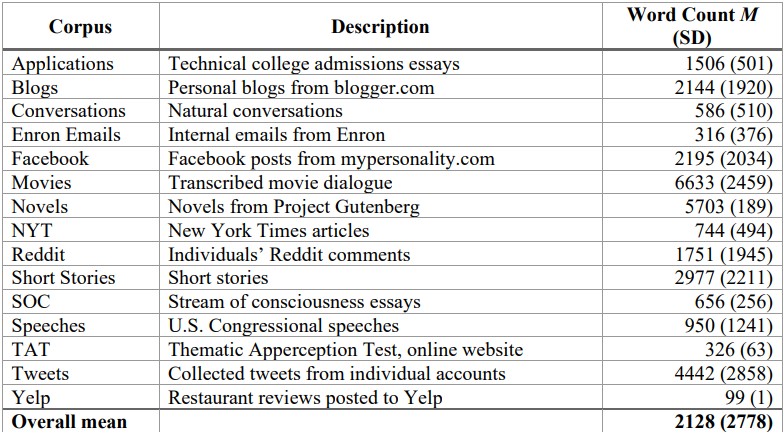
\includegraphics[scale=0.65]{./figures/test-kitchen-corpus.png}
	\caption{The test Kitchen Corpus of 31 Million Words \cite{boyd2022development}}
	\label{FigKitchenCorpus}
\end{figure}

\subsection{Assessing LIWC-22's Accuracy}

\quad The process of quantifying the reliability and validity of text analysis tools like LIWC-22 presents unique challenges, different from the conventional approaches used in psychological assessments. The differences between verbal behavior and structured questionnaire responses needs a nuanced approach to evaluating the properties of LIWC categories.

Unlike self-report questionnaires that measure emotions like anger, sadness or ability to cooperate, through multiple, similar questions to ensure internal consistency, natural language does not conform to such repetitive patterns. In real-world communication, be it a social media post, an essay, or a conversation, individuals express a thought and then naturally progress to the next. This characteristic of verbal expression implies that the standards applied to language-based analyses must be adjusted to account for the unique dynamics of verbal behavior \cite{boyd2022development}.

The evaluation of LIWC-22's reliability involves an innovative adaptation to the language's non-repetitive nature. Taking the LIWC-22 Anger scale as an instance, the scale encompasses 181 words and phrases associated with anger. Theoretically, the usage of one anger-related word in a text should correlate with the usage of other anger-related words within the same text. By analyzing how each of these words is employed across a selection of texts and calculating the intercorrelations among these word usages, LIWC-22's approach to determining internal consistency emerges\cite{boyd2022development}.

Validating the numerous LIWC dimensions poses a significant and complex challenge. By their nature, LIWC's content categories appear to be directly relevant or face valid. Yet, the deeper question lies in determining the extent to which both personal and social psychological processes are mirrored in the use of language. For instance, the implications of using words related to "affiliation" at a high frequency raise questions about the user's social connections and needs. Are individuals using these words seeking more social interaction, or do they reflect a person's existing strong social ties? Additionally, it is important to consider whether the frequency of such language usage offers insights into or predictions about someone's social relationships and needs.

To compute these metrics, LIWC-22 employs two statistical methods: the Cronbach’s alpha (\textalpha) for continuous data, based on the percentage of total words, and the Kuder–Richardson Formula 20 (KR-20) for binary data \cite{kuder1937theory}, indicating the presence or absence of words. The application of Cronbach’s alpha in the context of LIWC-22 encounters a problem due to the variable base rates of word usage within language categories. This variability can lead to underestimations of reliability when using traditional methods. Conversely, the Kuder–Richardson Formula 20 offers a more accurate reflection of a category's internal consistency by accommodating the binary nature of word presence, thus providing a better approximation of reliability in language analysis.

In 2021, there was a great amount of research combining text analysis and social and psychological behaviors, with more than 2,400 studies using LIWC to examine text. Findings from these studies, including those from the developers' own laboratories, reveal correlations between the affect or emotion categories detected by LIWC in texts and the authors' self-reported feelings. These correlations, although modest, show the tool's capability to capture psychological dynamics to a certain extent. Higher correlations are observed when comparing judges' ratings of writing samples with LIWC scores, suggesting a somewhat consistent external validation of LIWC's analytical output\cite{boyd2022development}.